
\chapter{Implementation}
\label{chap:implementation}
% logo definitions
\newcommand{\logoFleur}{%
  \begingroup\normalfont
  
\includegraphics[height=1.2\fontcharht\font`\B]{img/logo/fleur.png}%
  \endgroup
}
\newcommand{\logoAiida}{%
  \begingroup\normalfont
  
\includegraphics[height=1.0\fontcharht\font`\B]{img/logo/aiida.png}%
  \endgroup
}
\newcommand{\logoAiidalab}{%
  \begingroup\normalfont
  
\includegraphics[height=1.0\fontcharht\font`\B]{img/logo/aiidalab.png}%
  \endgroup
}
\newcommand{\logoBinder}{%
  \begingroup\normalfont
  
\includegraphics[height=1.2\fontcharht\font`\B]{img/logo/binder.png}%
  \endgroup
}
\newcommand{\logoBokeh}{%
  \begingroup\normalfont
  
\includegraphics[height=1.2\fontcharht\font`\B]{img/logo/bokeh.png}%
  \endgroup
}
\newcommand{\logoDash}{%
  \begingroup\normalfont
  
\includegraphics[height=1.2\fontcharht\font`\B]{img/logo/dash.png}%
  \endgroup
}
\newcommand{\logoDocker}{%
  \begingroup\normalfont
  
\includegraphics[height=1.2\fontcharht\font`\B]{img/logo/docker.png}%
  \endgroup
}
\newcommand{\logoHoloviews}{%
  \begingroup\normalfont
  
\includegraphics[height=1.2\fontcharht\font`\B]{img/logo/holoviews.png}%
  \endgroup
}
\newcommand{\logoHvplot}{%
  \begingroup\normalfont
  
\includegraphics[height=1.2\fontcharht\font`\B]{img/logo/hvplot.png}%
  \endgroup
}
\newcommand{\logoJavascript}{%
  \begingroup\normalfont
  
\includegraphics[height=1.2\fontcharht\font`\B]{img/logo/javascript.png}%
  \endgroup
}
\newcommand{\logoJupyter}{%
  \begingroup\normalfont
  
\includegraphics[height=1.2\fontcharht\font`\B]{img/logo/jupyter.png}%
  \endgroup
}
\newcommand{\logoMatplotlib}{%
  \begingroup\normalfont
  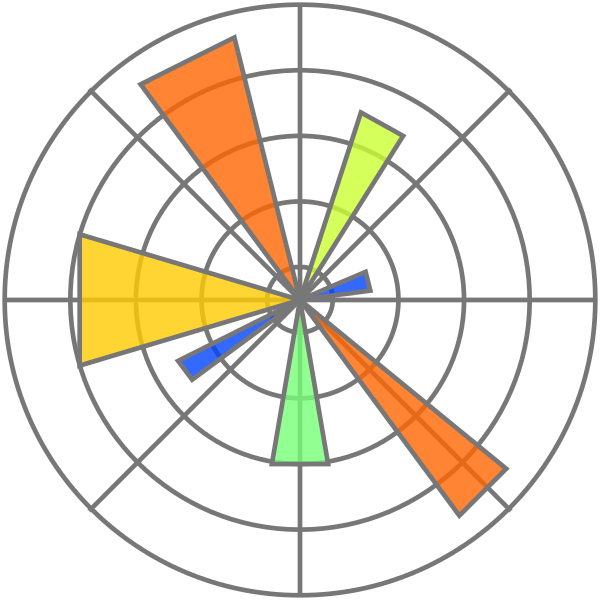
\includegraphics[height=1.2\fontcharht\font`\B]{img/logo/matplotlib.png}%
  \endgroup
}
% \newcommand{\logoMpld3}{%
%   \begingroup\normalfont
%   
\includegraphics[height=1.2\fontcharht\font`\B]{img/logo/mpld3.png}%
%   \endgroup
% }
\newcommand{\logoPanel}{%
  \begingroup\normalfont
  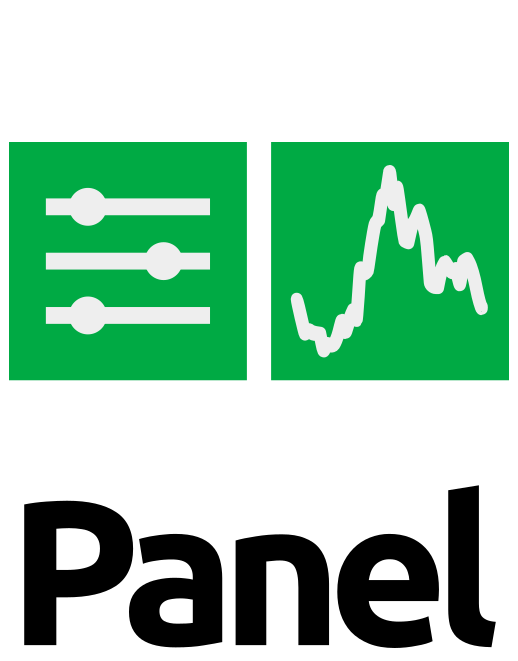
\includegraphics[height=1.2\fontcharht\font`\B]{img/logo/panel.png}%
  \endgroup
}
\newcommand{\logoParam}{%
  \begingroup\normalfont
  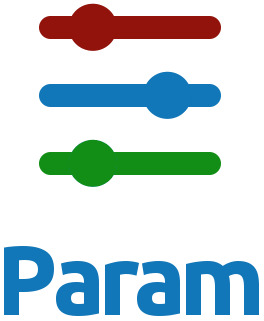
\includegraphics[height=1.2\fontcharht\font`\B]{img/logo/param.png}%
  \endgroup
}
\newcommand{\logoPlotly}{%
  \begingroup\normalfont
  
\includegraphics[height=1.2\fontcharht\font`\B]{img/logo/plotly.png}%
  \endgroup
}
\newcommand{\logoPython}{%
  \begingroup\normalfont
  
\includegraphics[height=1.2\fontcharht\font`\B]{img/logo/python.png}%
  \endgroup
}
\newcommand{\logoPyviz}{%
  \begingroup\normalfont
  
\includegraphics[height=1.2\fontcharht\font`\B]{img/logo/pyviz.png}%
  \endgroup
}
\newcommand{\logoSeaborn}{%
  \begingroup\normalfont
  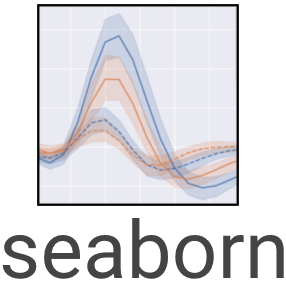
\includegraphics[height=1.2\fontcharht\font`\B]{img/logo/seaborn.png}%
  \endgroup
}

%%% Local Variables:
%%% mode: latex
%%% TeX-master: t
%%% End:


As per the requirements expounded upon in the introduction, the deliverable of
the project should be a finished software product. The software is written in
Python so as to integrate easily with the research groups ongoing software
projects around the Fleur code \cite{fleur}, chiefly \texttt{masci-tools}
\cite{masci-tools}, AiiDA \cite{aiida}. The clients split into frontend users
and code developers. In order to accommodate this, the product is organized into
three unidirectionally dependent subpackages or -modules, see Figure
\ref{fig:modules}.

An important design consideration was to account for unknown use cases. This has
been realized in each submodule by decoupling of \textbf{interface} and
\textbf{implementation}. The interfaces do not rely on any specific input file
format, visualization method or package, unlike the implementations for a
specific task or \emph{application}. The application in the scope of this
project are the band structure and density of states visualization, and for
these, this project provides a few implementations.

This design choice was also one reason why the product does not reuse any of the
\texttt{masci-tools} routines which partly solve quite similar problems, but
seemed to be to specialized in an initial code review. For these developers, one
added value of the project product could be to inspire the integration in a
common interface, where the current abstraction level could only be a starting
point.

\begin{figure}[htb!]
    \centering
    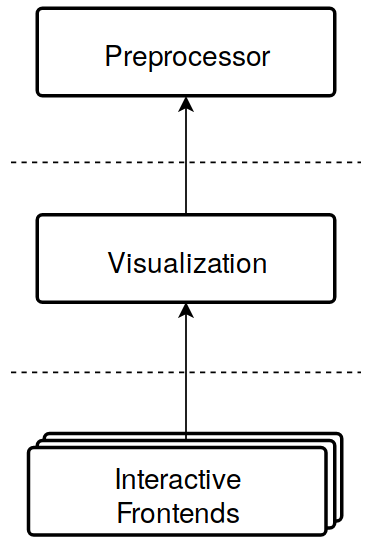
\includegraphics[width=0.3\linewidth]{img/module_design.png}
    \caption{Module Design}
    \label{fig:modules}
\end{figure}

\section{Preprocessor Module}
\label{sec:preprocessor-module}

This is the 'backend' of the tool. It is basically a file reader for the input
data, the Fleur simulation output. The formats are the Hierarchical Data Format
(HDF) \cite{hdf} for the band structure, and a Fleur-specific simple
comma-separated values (CSV) format for the density of states (DOS).

The HDF format is basically a binary flexible container for all kinds of common
binary and text file formats, each of which constitutes a \textbf{dataframe}
inside the HDF file. The format supports metadata annotation and high-throughput
input/output (I/O). As a consequence, it is considered by some developers in
some application domains which rely on numerical simulation codes to be one
possible base for the establishment of common domain-specific rich data exchange
standards in order to increase code interoperability. These developers are in
the process of extending their codes' I/O capabilities towards that end.
However, HDF's flexibility comes at the cost of a relatively complex Application
Programming Interface (API) as the keyhole for all operations.

The preprocessor module tries to hide that complexity by offering the
\texttt{Recipe} interface, see Figure \ref{fig:preprocessor}. One
\texttt{Recipe} is a dictionary that describes a complete
\href{https://en.wikipedia.org/wiki/Extract,_transform,_load}{Extract-Transform-Load}
(ETL) pipeline for one specific application. UAREHERE

\begin{figure}[htb!]
    \centering
    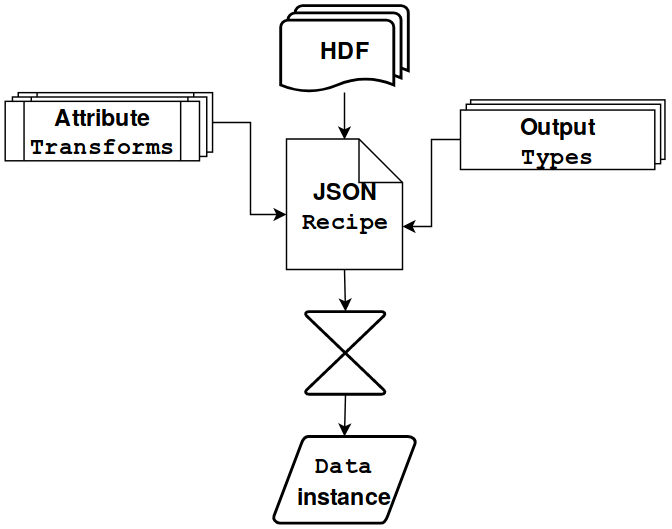
\includegraphics[width=0.6\linewidth]{img/reader_flowchart4.png}
    \caption{The preprocessor module.}
    \label{fig:preprocessor}
\end{figure}

\section{Visualization Module}
\label{sec:visualization-module}

\section{Frontend Modules}
\label{sec:frontend-modules}

\subsection{Desktop Frontend}
\label{sec:desktop-frontend}

\subsection{Web Frontend}
\label{sec:web-frontend}





%%% Local Variables:
%%% mode: latex
%%% TeX-master: "../report"
%%% End:

%  LocalWords:  subpackages submodule
